\documentclass[a4paper,12pt]{article}
\usepackage[utf8]{inputenc}
\usepackage[T1]{fontenc}
\usepackage[magyar]{babel}
\usepackage{indentfirst}
\usepackage{amsmath}
\usepackage{graphicx}
\frenchspacing
\author{Belényesi Roland}

\begin{document}
\section{Bevezetés}
A big data napjainkban az egyik vezető címke az informatikai terminológiák körében, különböző címekkel ellátva, mint: 
\textsl{Sikerhez és boldogsághoz vezet a big data}~\cite{ori} vagy 
\textsl{Új korszak kezdődött a tudományban.}~\cite{oria} De mit is jelent pontosan? Nincs explicit kimondott meghatározás a fogalomra, de Doug Laney 2001-es definíciója egy jó kindulópontnak tekinthető: az adatok nagy mennyiségben (volume), gyorsan(velocity) és különböző formátumban(variety) jelennek meg (3V's)~\cite{3v}.Azonban, ma már kiegészíthetjük ezt a fogalmat még 2V-vel: bizonyosság(veracity) és érték(value).~\cite{5v} Az adatmennyiség amit előállítunk exponenciálisan növekszik olyan szintre, aminek tárolását, menedzselését és elemzését már nem tudjuk megoldani a saját, lokális erőforrásainkon belül az eddig megszokott adatelemzési eszközökkel, mint például Microsoft Excel, vagy különböző relációs adatbázis technológiák által.
Becslések~\cite{2020} szerint az adatok mennyisége kétévente duplázódik, így 2020-ra az összekézben forgó adatmennyiség elérheti a 44 zetabájtnyi (vagy 44 trillió gigabájtnyi) mennyiséget.
\linebreak

A "big data" lehetőséget biztosít arra, hogy ezeket az adatokat ne csak tároljuk, hanem új módokon tanuljunk belőle, értéket állítsunk elő, többet megtudjunk ügyfeleinkről, a saját üzleti folyamatainkról, ami versenyelőnyhöz vezethet. E mellett az áttörő kutatások számát is megnöveli azáltal, hogy rejtett összefüggéseket mutat meg.~\cite{brk} 

A cloud computing, és új technológiák megszületése és az, hogy a fizikai világ egyre jobban átterelődik az online térbe, új nehézségeket állít elő mind az adatokat kiszolgáló, mind az adatokat elemző infrastruktúrák számára. Ezek a problémák komoly gondot jelentek az informatikai iparnak, mivel érintik az fizikai manifesztációt (hardver), mind az ezt vezérlő és feldolgozó réteget (szoftver és algoritmus). Ezek a problémák,~\cite{dst} --amelyek a tradícionális adattárház technológiákra jellemzőek-- többek között származhatnak a hiba-tolerancia hiányából, a sokféle adatfajtából,a párhuzamosság hiányából, mely azt eredményezi, hogy a mai technológia fejlettség (és a központi számítási egységek fizikailag limitáltsága miatt) nem lesz megfelelő számítási teljesítmény a megnövekedett adatmennyiség menedzselésére.

\section{A dolgozat célja}

A technológia fejlődése és a számítási teljesítmény megnövekedése hozta létre azt az üzleti igényt~\cite{rta}, hogy egyre gyorsabban, egyre nagyobb adatmennyiség feldolgozása történjen meg. Ilyen igény például:csalás felderítés~\cite{fraud}, "dolgok" internete (IoT)~\cite{iot} vagy alkalmazás monitoring~\cite{ganalitycs}. Ez az adatfeldolgozási sebesség olyan szintre eljutott, hogy közel valós időben, az adat keletkezése után megtörténhet ennek feldolgozása. Ilyen gyorsaságú adatfeldolgozásra csak elosztott rendszerek segítségével vagyunk képesek,~\cite{ucl} amelyek felépítésükből fakadóan sok lehetőség és költség jellemez, amelyeket a későbbiekben fogok kifejteni. A dolgozatomban használt Apache Flink (mely az Apache Foundation egyik legújabb és legmodernebb terméke) platform közel 40 millió elem feldolgozására képes egy 40 magos architektúrán másodpercenként.~\cite{flink}.  \linebreak

Ahhoz, hogy ezt az adatmennyiséget ki tudjuk elemezni és ajánlásokat tudjunk adni, gépi tanulásra van szükségünk. A gépi tanulás az informatikának és a matematikának egy olyan ága, amely az adatok folyamatos betáplálása során új ismereteket szolgáltat, megpróbál előrejelzéseket adni anélkül, hogy explicit módon be lenne erre programozva. ~\cite{ml}. A választott metódus a stochastic gradient descent (SGD, sztochasztikus gradiens ajánlás)~\cite{sgd}, amely egy olyan egyszerűsítési illetve optimalizációs eljárás, ahol adott célfüggvény gradiensét folyamatosan, iteratív módon számoljuk ki. Célom az, hogy megtervezzem Apache Flink alatt az SGD algoritmust, összehasonlítsam a teljesítményét a már implementált algoritmusokkal és megkezdjem a szükséges módosítások implementálást.

\section{Gépi tanulás}

Amikor tanulunk, a célünk, hogy minél jobb eredményeket érjünk el a számonkérésen, vagy minél több tudást halmozzunk fel, amit a későbbiek során (valószínűsíthetően) hasznosítani tudunk. A gépi tanulásnak is ugyanez a célja, különböző modellek megalkotása után a megadott példákból (input adat) különböző kimeneteket (output adat) ad ki. Az input adatokból próbál általánosítani oly módon, hogy az felhasználható legyen számára ismeretlen problémák során. Gépi tanulást használunk például: 
\begin{itemize}
\item web keresés
\item spam szűrés
\item ajánló rendszerek
\item online hírdetések
\end{itemize}
esetén is. 
Egy 2011-es Mckinsey riport ~\cite{mckinsey} szerint a gépi tanulás (illetve a prediktív analitika) lesz a következő évek innovációinak alapja. IBM Watson-ja~\cite{watson}, már képes a beadott tünetek alapján, megjósolni, hogy mi lehet a páciens betegsége (egyelőre még csak fejlesztőknek, API-n keresztül). \linebreak

Két fő csoportja van a gépi tanulási algoritmusoknak: a felügyelt (supervised) és nem felügyelt (unsupervised) tanítás.

\subsection{Felügyelt tanítás}

Általánosan fogalmazva, az adat amit betáplálunk a gépi tanulás modellünkbe, tréning példáknak (training set) nevezzük. A tréning példák $x$, $y$ párokat tartalmaznak, ahol $x$ az érték vektor (feature vector). Minden $x$ érték: kategórikus (diszkrét értékeksorozatból származik, pl{kék, piros, sárga}) vagy numerikus (az érték egész vagy valós szám). $y$ a címke (label), ami kategorizáló érték $x$-re nézve.A célünk az, hogy felfedezzük azt az 
\begin{equation*} y=f(x)
\end{equation*}
függvényt, ahol a legjobban előre tudjuk jelezni az $y$ értéket a meghatározott $x$-re nézve.

Fontos, hogy szétválasszuk az adatainkat tréning és teszt adatokra. Ez biztosítja azt, hogy ne fordulhasson elő az a probléma, hogy a modellünk túlságosan fontos súllyal vesz egyes objektumokat az adatsoron (amik nem jellemzőek a lehetséges valós adatokra), ami azt eredményezi, hogy a valós problémákon már nem fog eredményesen működni. A problémát túltanulásnak vagy magolásnak (overfitting) nevezik.\~cite{overfit}


\begin{figure}[ht!]
\centering
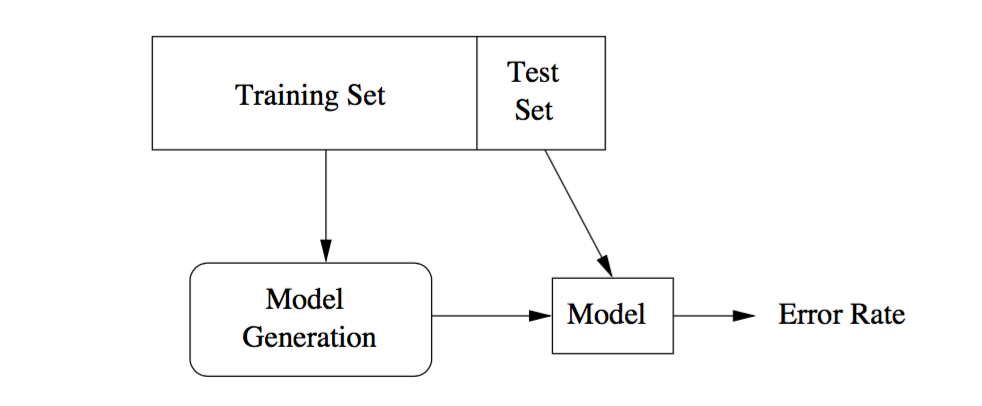
\includegraphics[width=90mm]{img/ml.png}
\caption{Felügyelt tanulás általános modellje \label{overflow}}
\end{figure}

\subsection{Nem felügyelt tanítás}
Nem felügyelt tanítás esetén adottak: $(x_1, x_2, ..., x_n)$ adataink, és nincs célfüggvényünk, vagy elvárt kimenetünk. Alapvetően nem struktúrált \textsl{zajból} próbálunk mintázatot keresni, olyan modellt létrehozni, ami jól reprezentálja adatok valószínűségi eloszlálást. Annak ellenére, hogy nincs információnk arról, hogy az egyes adatok milyen kapcsolatban vannak egymással, $(x_t)$ valószínűségi eloszlását meg tudjuk jósolni  $(x_1,x_2, ..., x_{t-1})$ alapján, ahol $P(x_t|x_1,x_2, ..., x_{t-1})$.
Egyszerűbb esetekben, ahol az bemenet sorrend irreleváns, lehet modellt építeni az adatra, ahol $(x_1, x_2, ...)$ az adatsorunk, és ezek függetlenül de identically származnak a $P(x)^2$-ból.~\cite{unsupervised}

\section{Ajánlórendszerek}
Az ajánlórendszerek olyan, főként webes rendszerek, ahol a különböző forrásból származó adatok alapján ajánlunk olyan lehetőségeket a felhasználóknak, ami nagy valószínűséggel megfelel a preferenciájának. Például:
\begin{itemize}
\item Youtube, ahol az nézettségi történet alapján kapja az ajánlásokat a felhasználó
\item Netflix, ahol az a cél, hogy a felhasználónak olyan sorozatokat ajánljunk, amit nagy valószínűséggel kedvelni fog
\end{itemize}
Két fő fajtáját különböztetjük meg az ajánló rendszereknek. A Content-based (tartalom alapú) ahol az item tulajdonságait vizsgáljuk, illetve a collaborative filtering (együttműködésen alapuló szűrés), ahol a hasonló érdeklődésű felhasználóknak nyújtott ajánlásokat vesszük alapul. \linebreak

Az ajánlórendszerek alapja az ún. utility matrix, ami tartalmazza a felhasználókat és hozzájuk kapcsolt elemek adatait. Minden felhasználó-item párhoz egy értéket rendelünk, ami jellemzi, hogy mennyire preferálja az adott elemet. Ez az érték általában egy rendezett skáláról (pl.: 5 elemű skála, 1-től 5-ig számozva, ahol az 1 a legkevésbé, az 5 pedig a legjobban kedvelt elemet jelöli) kerül ki. Alapfeltevés, hogy a mátrixunk ritka (nincs teljesen kitöltve), mivel nem értékel minden felhasználó minden elemet. A hiányzó, nem ismert értékekről semmilyen explicit információval nem rendelkezünk.

\begin{figure}[ht!]
\centering
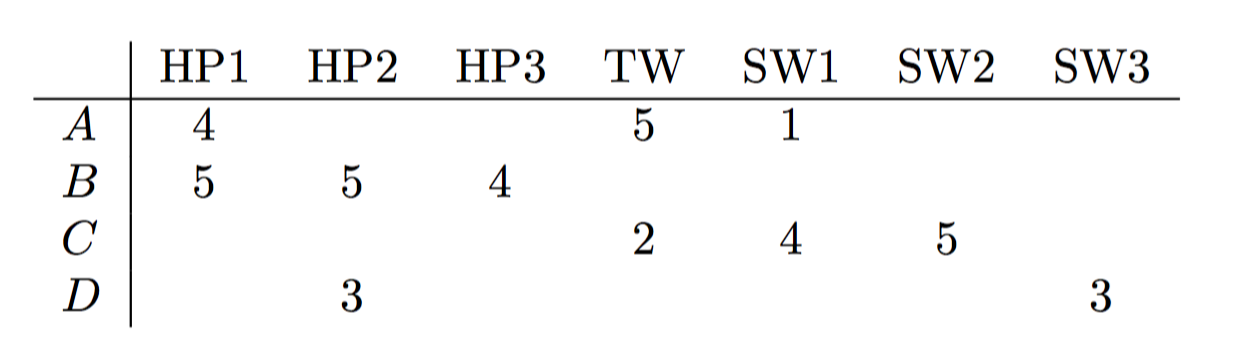
\includegraphics[width=90mm]{img/um.png}
\caption{Utility matrix, ahol az $A,B, C, D$ felhasználók a Star Wars, Harry Potter és Twilight filmeket értékelték \label{overflow}}
\end{figure}

Célünk az, hogy hiányzó értékeket a mátrixban minél jobban megjósoljuk. Természetesen nem fontos, hogy az összes elemét kitöltsük, törekednünk kell arra, hogy az ajánlás a preferált filmek/cikkek körében legyen, mivel ezek eladása/elolvasása racionalizálható gazdasági szempontból. Jelen esetben, kíváncsiak lehetünk, hogy $A$ felhasználónak ajánlhatjuk-e Harry Potter 2. részét. Láthatjuk, hogy HP 1. részét kedvelte, és tudjuk, hogy a két film kapcsolatban van egymással (rendezők, színészek, történet, stb.) ezért gyaníthatjuk, hogy a második részt is jól fogja értékelni.

\subsection{Long Tail}

Amikor bemegyünk egy könyvesboltba, többféle módon is választhatunk egyes könyvek közül. Vannak kiemelt könyvek, amikre nagy az érdeklődés, ezért a könyvesbolt jobban reklámozza ezeket. Személyes ajánlásra nincs lehetőség, a választék korlátozott, erőforrás hiányában az összes könyvnek csak egy szűk szeletét mutatja meg egy könyvesbolt. Ezzel szemben egy online bolt bármit ajánlhat, ami létezhet, nem csak a populárisabbakat, hanem a kevésbé keresetteket is. Ezt a megkülönböztetést nevezzük \textsl{long tail}-nek~\cite{longtail}, és ez az, ami létrehozta az ajánlórendszerek igényét. Muszáj ajánlanunk a felhasználónak termékeket --mivel nincs olyan nyilvánvaló módon prezentálva, mint a fizikai boltoknál-- ahhoz, hogy nagyobb eséllyel vásároljon belőlük.

\subsection{Utility mátrix feltöltése}
Utilty mátrix nélkül nem lehetséges a felhasználóknak ajánlattétel. Ahhoz, hogy feltudjuk tölteni, két általános megközelítés létezik.
\begin{enumerate}
\item Megkérdezzük a felhasználót a véleményéről (pl.: IMDb, ahol a felhasználók a filmeket értékelhetik egy 1-10-es skálán:)~\cite{imdb}: Ebben az esetben a sikerességünk limitált, mivel a felhasználónak nem származik rövid távon gazdasági előnye abból, hogy értékel (természetesen, ha minden film után reális értékelést adna, akkor hosszú távon jobb ajánlásokat kapna). Másrészt az emberi irracionalitás miatt előfordulhat, hogy részrehajlóan (akár pozitív, akár negatív irányban) értékel, ami eltorzíthatja a utility mátrixot. ~\cite{introspection}
\item Megvizsgáljuk a viselkedését: ebben az esetben azt vizsgáljuk, hogy a felhasználó megtekintette/megvette/stb. az adott terméket. Ha igen, explicit 1-el töltjük fel a mátrixot, ha nem akkor 0-val. Tehát, ha megveszünk (vagy csak megnézünk) egy könyvet az Amazonon, akkor 1-el fogja értékelni a utility mátrixban az ajánló rendszer. Így kiküszöbölhetjük azt, hogy a felhasználó, nem szeretne vagy nem tud helyesen értékelni. Hátránya, hogy nehéz súlyozni a különböző véleményeket, mivel csak 1 elemű skálán dolgozunk.
\end{enumerate}

\section{Párhuzamos kötegelt feldolgozás}
A kétezres évek elején és közepén, a megfelelő számítási kapacitás hiányában a párhuzamos adatfeldolgozás általában \textsl{kötegelt} (batch) módon történt. Felhasználói interakció nélkül, megadott időközönként történik a nagy mennyiségű adat feldolgozása. Előnye, hogy akkor futhat a program, amikor a rendszer leterheltsége alacsony, ezzel biztosítva az egyenletes kihasználtságot. Mivel a parancsok automatikusan futnak le, ezért kisebb az üres, nem számítással töltött idő.~\cite{batch}

\section{Lambda-architektúra}
A big data megjelenésével, megjelent az igény, hogy ezeket az adatokat közel valós időben tudjuk feldolgozni. Egy fejlettebb megoldásnak tekinthetjük a Lambda-architektúrát, ami a kötegelt feldolgozást (batch processing), és a adatfolyam feldolgozást (stream processing) egyesíti. Megalkotása során törekedtek arra, hogy 
\begin{itemize}
\item robosztus, hiba toleráns legyen, mind hardver, mind szoftver oldalon
\item széles körű felhasználhatóság biztosítson, alacsony válaszidővel
\item horizontálisan skálázható legyen (több "általános célű" gép használatával lehessen növelni a teljesítményt)
\item bővíthető legyen
\end{itemize}

Ezen feltételek mellett egy három rétegű architektúrát alkotott meg Nathan Marz~\cite{lambda}. A kötegelési réteg (batch layer), a sebesség réteg (speed layer) és a kiszolgáló réteg (serving layer) biztosítja az adatfeldolgozást. Az adat változatlan formában eljut mind a kötegelt, mind a sebesség rétegbe. A kötegelt réteg tartalmazza a mester adathalmazt, ami nem módosítható, csak egyszer írható formában tárolja az adatokat. Ez a réteg meghatározott időszakonként, ciklikusan lefutattja a számításait, amivel létrehozza az ún. kötegelt nézetet (batch view). Ez a réteg felel azért, hogy az adat pontosan (lehetséges újraszámítás, ahogy érkeznek az újabb adatok) és teljesen jelenjen meg a felhasználó előtt (magas válaszidővel).  A kiszolgáló réteg indexeli ezeket a nézeteket, ezzel biztosítva az ad-hoc, gyors lekérdezéshetőségüket. \linebreak
A sebesség réteg csak friss adatokkal dolgozik, így csökken a pontosság és a teljesség, viszont gyors, inkrementális algoritmusok segítségével, alacsony válaszidővel tudja az adatokat a kimenetre küldeni. A kiszolgáló réteg a kötegelt és a sebesség nézetek összefűzéséből állítja elő az elvárt kimenetet.

\begin{figure}[ht!]
\centering
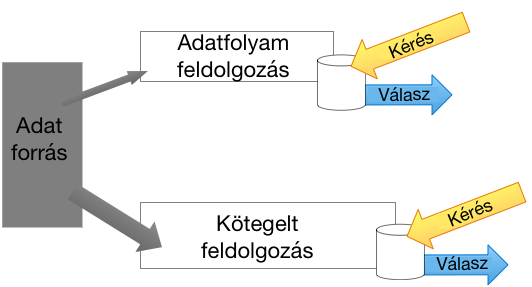
\includegraphics[width=90mm]{img/lambda.png}
\caption{Lambda architektúra felépítése \label{overflow}}
\end{figure}

\section{Adatfolyam}
bounded, unbounded

\iffalse
\section{Time-agonistic}
\begin{itemize}
\item Event time
\item Proccesing time
\end{itemize}
\section{Flink(Spark/Storm/Mapreduce)}
\section{Ajánlórendszerek}
\begin{itemize}
\item Collaborative filtering
\item Content based
\end{itemize}
\section{ALS}
\section{DSG}
\section{Java, Scala}
Max 1 oldal, miért ez lett
\section{Dcg,nDCG}
\fi

\end{document}

\begin{thebibliography}{99}
\bibitem{ori}http://www.origo.hu/techbazis/20151020-big-data-adatok-elemzes-siker-ceg-startup.html, Megtekintve: 2015.12.14
\bibitem{oria}http://www.origo.hu/tudomany/20131014-big-data-adatelemzes-tudomany-adatbanyaszat-informatika.html, Megtekintve: 2015.12.14
\bibitem{3v}http://blogs.gartner.com/doug-laney/files/2012/01/ad949-3D-Data-Management-Controlling-Data-Volume-Velocity-and-Variety.pdf, Megtekintve: 2015.12.15
\bibitem{5v}http://enterprisearchitects.com/the-5v-s-of-big-data/, Megtekintve: 2015.12.15
\bibitem{log}http://www.infoworld.com/article/2608064/big-data/big-data-log-analysis-thrives-on-machine-learning.html, Megtekintve: 2015.12.15 
\bibitem{brk}http://www.informationweek.com/government/big-data-analytics/big-data-disease-breakthroughs/d/d-id/1316310, Megtekintve: 2015.12.15
\bibitem{2020}http://www.emc.com/leadership/digital-universe/2014iview/executive-summary.htm, Megtekintve: 2015.12.15
\bibitem{sas}http://www.sas.com/en_us/insights/articles/big-data/big-data-and-iot-two-sides-of-the-same-coin.html, Megtekintve: 2015.12.15
\bibitem{dst}http://www.bogotobogo.com/WebTechnologies/distributedcomputing.php, Megtekintve: 2015.12.15
\bibitem{rta}https://en.wikipedia.org/wiki/Real-time_business_intelligence, Megtekintve: 2015.12.15
\bibitem{fraud}http://www.pactera.com/resources/blog/how-big-data-is-revolutionizing-fraud-detection-in-financial-services/, Megtekintve: 2015.12.15
\bibitem{iot}https://datafloq.com/read/real-time-analytics-internet-of-things/943, Megtekintve: 2015.12.15
\bibitem{ganalitycs}https://support.google.com/analytics/answer/1638635?hl=en, Megtekintve: 2015.12.15
\bibitem{ucl}http://www0.cs.ucl.ac.uk/staff/ucacwxe/lectures/ds98-99/dsee3.pdf, Megtekintve: 2015.12.15
\bibitem{flink}http://flink.apache.org/features.html#unified-stream-amp-batch-processing, Megtekintve: 2015.12.15
\bibitem{ml}http://www.sas.com/en_us/insights/analytics/machine-learning.html, Megtekintve: 2015.12.16
\bibitem{sgd}http://research.microsoft.com/pubs/192769/tricks-2012.pdf, Megtekintve: 2015.12.16
\bibitem{mckinsey}http://www.mckinsey.com/insights/business_technology/big_data_the_next_frontier_for_innovation, Megtekintve: 2015.12.16
\bibitem{watson}http://www-03.ibm.com/innovation/us/engines/assets/9442_Watson_A_System_White_Paper_POW03061-USEN-00_Final_Feb10_11.pdf, Megtekintve: 2015.12.16
\bibtem{overfit}Jure Leskovec, Anand Rajaraman, Jeffrey D. Ullman. (2014): Mining Of Massive Datasets, pp. 462.
\bibitem{unsupervised}http://mlg.eng.cam.ac.uk/zoubin/papers/ul.pdf, Megtekintve: 2015.12.16
\bibtem{recsys}Jure Leskovec, Anand Rajaraman, Jeffrey D. Ullman. (2014): Mining Of Massive Datasets, pp. 307-325.
\bibitem{longtail}http://knowledge.wharton.upenn.edu/article/rethinking-the-long-tail-theory-how-to-define-hits-and-niches/, Megtekintve: 2015.12.16
\bibitem{imdb}http://www.imdb.com/help/show_leaf?votestopfaq, Megtekintve: 2015.12.16
\bibitem{introspection} http://cbdr.cmu.edu/seminar/pronin.pdf, Megtekintve: 2015.12.16
\bibitem{batch}http://www-01.ibm.com/support/knowledgecenter/#!/zosbasics/com.ibm.zos.zmainframe/zconc_batchproc.htm,  Megtekintve: 2015.12.16
\bibitem{lambda}http://lambda-architecture.net, Megtekintve: 2015.12.16
\end{thebibliography}
